\documentclass{beamer}

% Theme
%\usetheme{Madrid}
%\usecolortheme{default}
\mode<presentation>
{
  \usetheme{Warsaw}
  \setbeamercovered{transparent}
}

\usetheme{Warsaw}

\setbeamersize{text margin left=3mm}
\setbeamersize{text margin right=3mm}

% Packages
\usepackage[utf8]{inputenc}
\usepackage[backend=bibtex, style=authoryear]{biblatex} % You can change the style if you prefer a different citation style
\addbibresource{Chp1.bib}

\usepackage{dirtytalk}
\usepackage{cancel}
\usepackage{graphicx}
\usepackage{wrapfig}
\usepackage{caption}
\usepackage{booktabs}

% Title slide
\title[]{Heterogeneous Returns and the Distribution of Wealth}
\author[Edwards]{Decory Edwards}
\institute[JHU]{Johns Hopkins University}
\date{\today}

\begin{document}

\begin{frame}
  \titlepage
\end{frame}

\section{Introduction}

\begin{frame}{Why do macroeconomists care about inequality?}

Empirical evidence shows that macroeconomic policies, as well as aggregate shocks, may have differential effects across households.

\begin{itemize}
\item Macro matters for inequality
\end{itemize}
\vspace{2.5mm}

Representative agent models have a difficult time matching empirical estimates of macroeconomic variables (MPC and the wealth distribution).

\begin{itemize}
\item Inequality matters for macro
\end{itemize}

%\cite{Ahn2017} note this two-way street between macroeconomics and inequality. Incorporating \textit{heterogeneity across households} can help with this second issue. 


\end{frame}

%\begin{frame}{Data on household wealth in the U.S.}
    
   % \begin{itemize}
    %\item Institute for Policy Studies (2019)
    %\begin{itemize}
    %	\item \say{In 2018, the total wealth of the poorest half of Americans was eclipsed by the combined wealth of the three wealthiest men in the nation.}
%	\item \say{The combined wealth of the top five richest men on this list skyrocketed by a staggering 123\% from March 2020 to October 2021.}
  %  \end{itemize}
    
    
  %  \item Trends in the composition of wealth holdings across households using Survey of Consumer Finances data \parencite{wolff2004}, \parencite{Wolff2021}
  %  \item Estimated distribution of wealth using IRS tax data for 1913 to 2012 \parencite{sz16}  
  %  \end{itemize}
    
%\vspace{2em}    
  %  Motivating question: What explains inequality in the distribution of wealth?
%\end{frame}
%%%%%%%%%%%%%

\subsection{Literature Review}
%\begin{frame}{Explaining inequality in the distribution of wealth}

 %   \cite{jbab18} provide a survey of historical thought and models describing mechanisms which lead to stationary, skewed distributions of wealth with heavy tails.
    
   % \vspace{1mm}
 %   \begin{enumerate}
   % \item Skewed distribution of earnings
    
%    \begin{itemize}
   % \small
 %   \item Edgeworth (1917), F.P.Cantelli (1921, 1929), Frechet (1939), D'Addario (1943), Mincer (1958), Lydall (1959), Kremer (1993)
  %  \vspace{1mm}
   % \item Gabaix and Landier (2008), Geerolf (2016)
  % \end{itemize}
    
  %  \item Stochastic returns to savings
    
  %  \begin{itemize}
  %  \small
   % \item Champernowne (1953), Kesten (1973)
  %  \end{itemize}
    
  %  \item Optimal consumption-saving behavior of individuals
  %  \end{enumerate}
 % \end{frame}
%%%%%%%%%%%%%%%%

\begin{frame}{Macro with heterogeneous agents}
    %Aim: Understand movements in macroeconomic aggregates by studying the collection of microeconomic (household) behavior.
    
    %\small
    \begin{itemize}
    \item Uninsurable, idiosyncratic risk to income and movements in aggregate productivity \parencite{ks1998} 
    \item Ex-ante heterogeneity in the time preference of households \parencite{cstw2017}
    \item Classifying models with ex-ante and ex-post heterogeneity \parencite{gkgv22}
    \item Further surveys regarding heterogeneous agent macroeconomics \parencite{Guvenen2011} and \parencite{Krueger2016} 
    \end{itemize}
    
\end{frame}
%%%%%%%%%%%%%%%%%%

\begin{frame}{Empirical estimates of returns}

   \small
   \begin{enumerate}
    \item Comprehensive, administrative tax data in Norway from 2004 to 2015  \parencite{aflgdmlp20}
    \item Asset holdings and income for Swedish residents from 1999 to 2007 \parencite{lblcps18}
    \item Wealth held in equity accounts in India from 2002 to 2011 \parencite{Campbell2019}
    \item DNB 2005 survey of dutch households regarding savings accounts and financial literacy \parencite{Deuflhard2018}
    \end{enumerate}
   
  
\end{frame}
%%%%%%%%%%%%%%%%%%


%\begin{frame}{Possible explanations for differences in returns}

 %  \small
   %\begin{itemize}
    %\item Entrepreneurial talent  
    
    %\parencite{Cagetti2008}
    
    %\item Financial knowledge/sophistication
    
    %\parencite{mkjnls19}, \parencite{alpmom17},  and \parencite{Lusardi2014}
    
    %\item Trust
    
    %\parencite{lgpslz2008} and \parencite{jbpglg2016}
    %\end{itemize}
  
%\end{frame}
%%%%%%%%%%%%%%%%%%

\begin{frame}{Related literature}
\begin{itemize}
\item Stochastic process for returns implying a stationary wealth distribution.
\par  \parencite{Benhabib2011}, \parencite{Benhabib2015}, \parencite{Benhabib2016}

\item Stochastic process for returns which best fits the empirical distribution of wealth.
\par \parencite{Benhabib2019}

\item Endogenize heterogeneous returns through access to high return investment technology.
\par  \parencite{Guler2022}
\end{itemize}
\end{frame}
%%%%%%%%%%%%%%%%%%%%%%%%
%Too many words here%
\begin{frame}{Outline}
\begin{enumerate}
\item Empirical evidence of heterogeneous returns
\item Model of saving with heterogeneous returns
\item Structural estimation of model to match wealth data
\end{enumerate}
\end{frame}
%%%%%%%%%%%%%%%%%%

\subsection{Heterogeneous Returns in the Data}
\begin{frame}{A closer look at \cite{aflgdmlp20}}
   
   \begin{columns}
     \column{0.5\textwidth}
     \small
     Following optimal portfolio choice theory from Merton (1969) and Samuelson (1969)
    \centering
    
    \begin{itemize}
    \item Optimal share in the risky asset is given by
    $$ \alpha_{it}^{m} = \frac{\mathbb{E}(r_{t}^{m} - r_{t}^{s})}{\gamma_i \sigma^{2}_{t}}.$$
    \item Individual \textit{realized} return to financial assets can be written as 
    $$ r_{it}^{f} = r_{t}^{s} + \alpha_{it}^{m} (r_{t}^{m} - r_{t}^{s}). $$
    \end{itemize}
    
    \column{0.5\textwidth}
    \centering
    \begin{figure}
    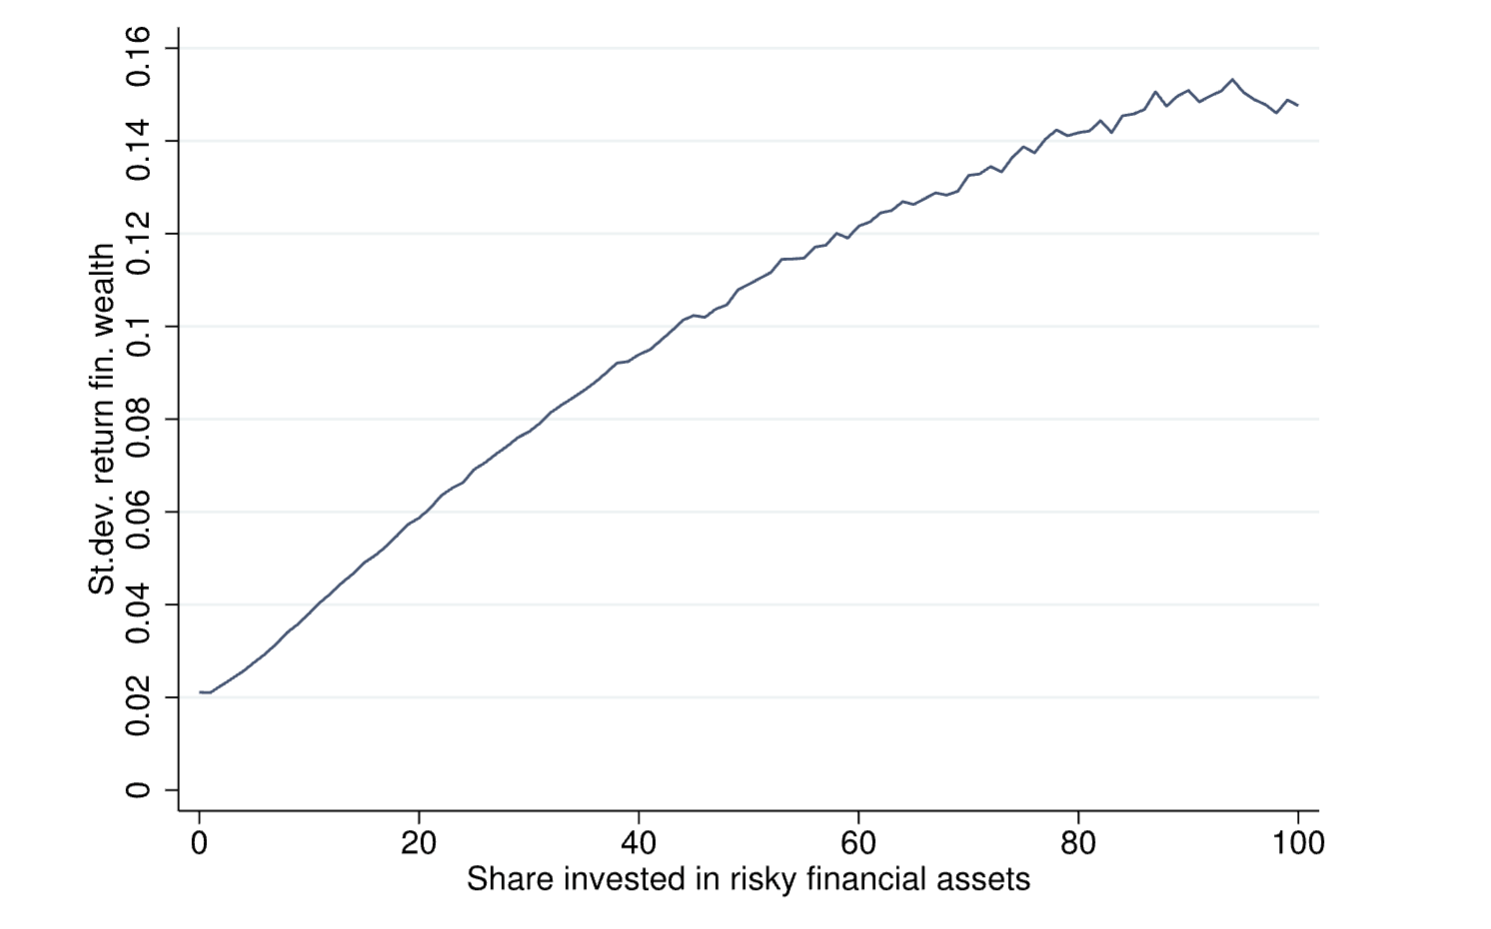
\includegraphics[width=\textwidth]{Figures/Fagereng2020Fig1.png}
    \captionsetup{font=scriptsize}
    \caption{Heterogeneity in returns to financial wealth by share of risky assets from \cite{aflgdmlp20}.}
    \end{figure}
  \end{columns}
   
\end{frame}
%%%%%%%%%%%%%%%%

\begin{frame}{}
   
     \begin{columns}
     \small
     \column{0.5\textwidth}
    \centering
    
    \begin{itemize}
    \item Step 1: \textit{linear panel data regression model} for the return to net worth
    $$ r^{n}_{it} = X^{'}_{it} \beta + u_{it}. $$
    \item Step 2: Add fixed effects 
    $$ u_{it} = f_{i} + e_{it}. $$
    $\implies R^2$ goes from $.33$ to $.5$.
    \end{itemize}
    
    
    \column{0.5\textwidth}
    \centering
    \begin{figure}
    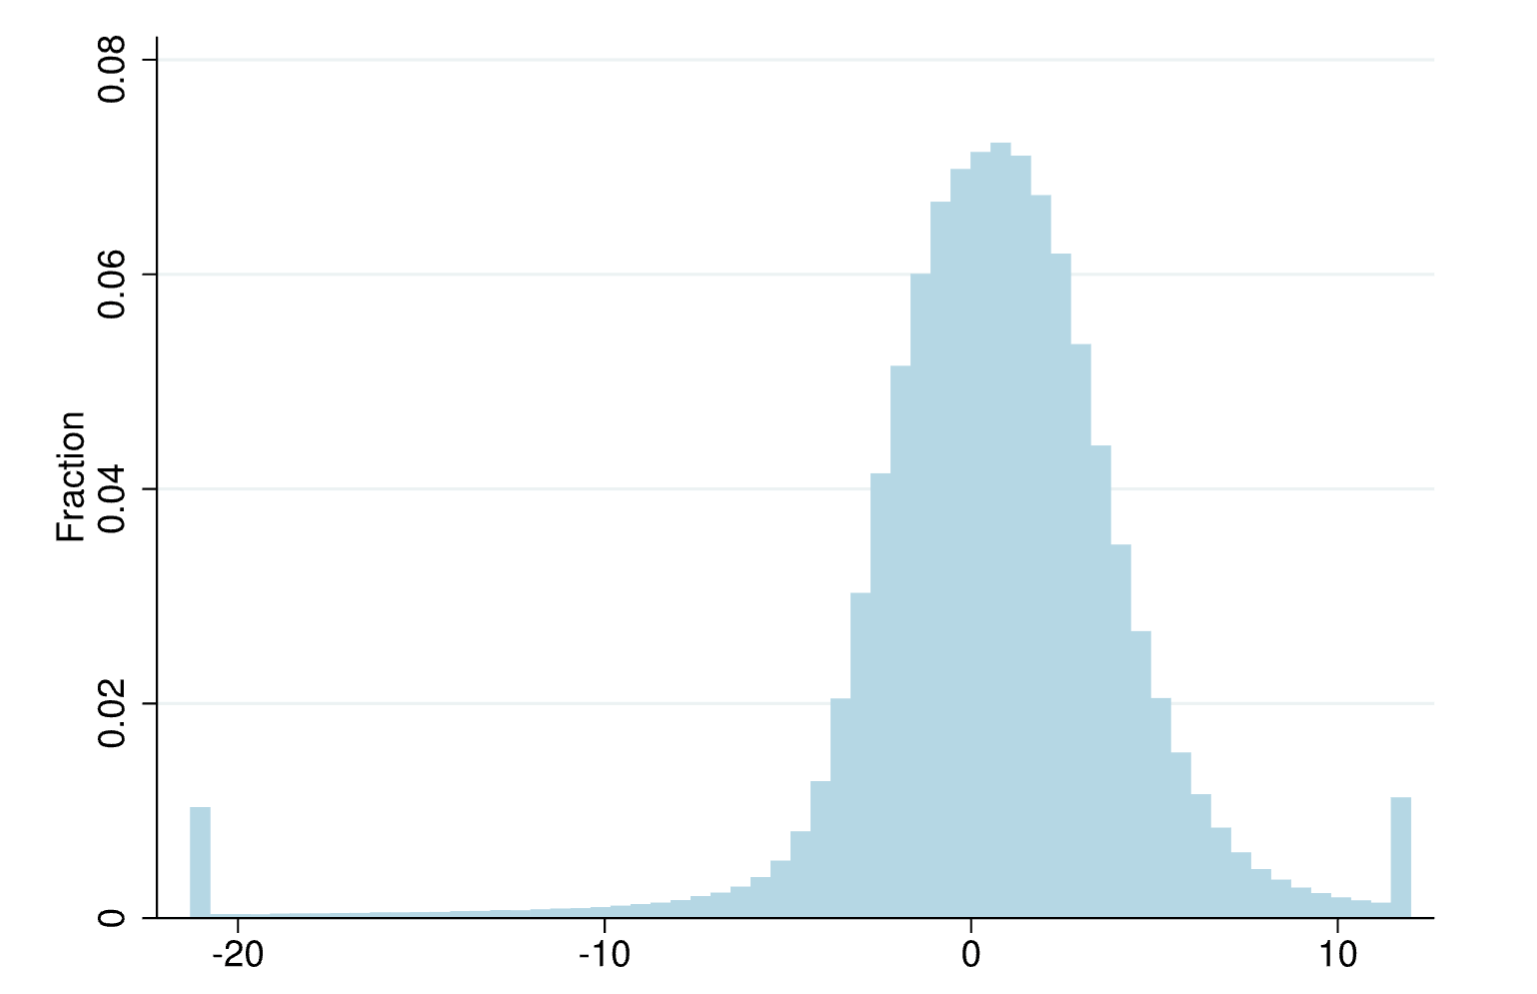
\includegraphics[width=\textwidth]{Figures/Fagereng2020Fig8.png}
    \captionsetup{font=scriptsize}
    \caption{Distribution of fixed effects in the return to net worth from \cite{aflgdmlp20}.}
    \end{figure}
  \end{columns}
   
\end{frame}
%%%%%%%%%%%%%%%%

\section{Model}
%\subsection{Environment}

\small
\begin{frame}{Labor income process}

\begin{itemize}
\item Household income: $$y_t = p_t \xi_t W_t$$
\item Permanent component: $$p_t = p_{t-1} \psi_t$$
\item Transitory component: $$\xi_t =
    \begin{cases}
       \mu & \text{with probability $\mho$} \\
      (1-\tau_t) l \theta_t & \text{with probability $1-\mho$}
   \end{cases}$$
\end{itemize}
%\vspace{1.5mm}

\end{frame}
%%%%%%%%%%%%%%%%%
%Put equations for permanent and transitory income%

\footnotesize
\begin{frame}{Heterogeneous agents in G.E.}

(Normalized) Optimization problem for households: Choose profiles $\{c_{t_n}\}_{n=0}^{\infty}$ that satisfy
 \begin{eqnarray*}
  v(m_t) &=& \max_{c_t} u(c_t(m_t)) + \beta \cancel{D} \mathbb{E}_{t}[\psi_{t+1}^{1-\rho}v(m_{t+1})] \\
  &\text{s.t.}& \\
  a_t &=& m_t - c_t(m_t), \\
  k_{t+1} &=& \frac{a_t}{\cancel{D}\psi_{t+1}}, \\
  m_{t+1} &=& (\daleth + r_t)k_{t+1} + \xi_{t+1}, \\
  a_t &\geq& 0.
\end{eqnarray*}

Production function $$Y = Z K^{\alpha} (\ell L)^{1-\alpha}$$ 

\end{frame}
%%%%%%%%%%%%%%%%%

%\begin{frame}{Rate of return and the evolution of market resources}
%\end{frame}
%%%%%%%%%%%%%%%%%

\begin{frame}{Conditions for a stable wealth distribution}

\cite{Carroll2019bst} provides the following \textit{death-modified growth impatience condition} such that a unique target wealth-to-permanent income ratio exists for households:

\begin{eqnarray*}
\left(\frac{(R \beta)^{1/ \rho}\mathbb{E}[\psi^{-1}]\cancel{D}}{\Gamma}\right) & < & 1.
\end{eqnarray*} 

\end{frame}
%%%%%%%%%%%%%%%%%

\subsection{Simulation}
%%%%%%%%%%%%%%%%%

\begin{frame}{Calibration}

Standard calibration scheme used to simulate the model.

  \vfill
   \begin{figure}
    \centering
    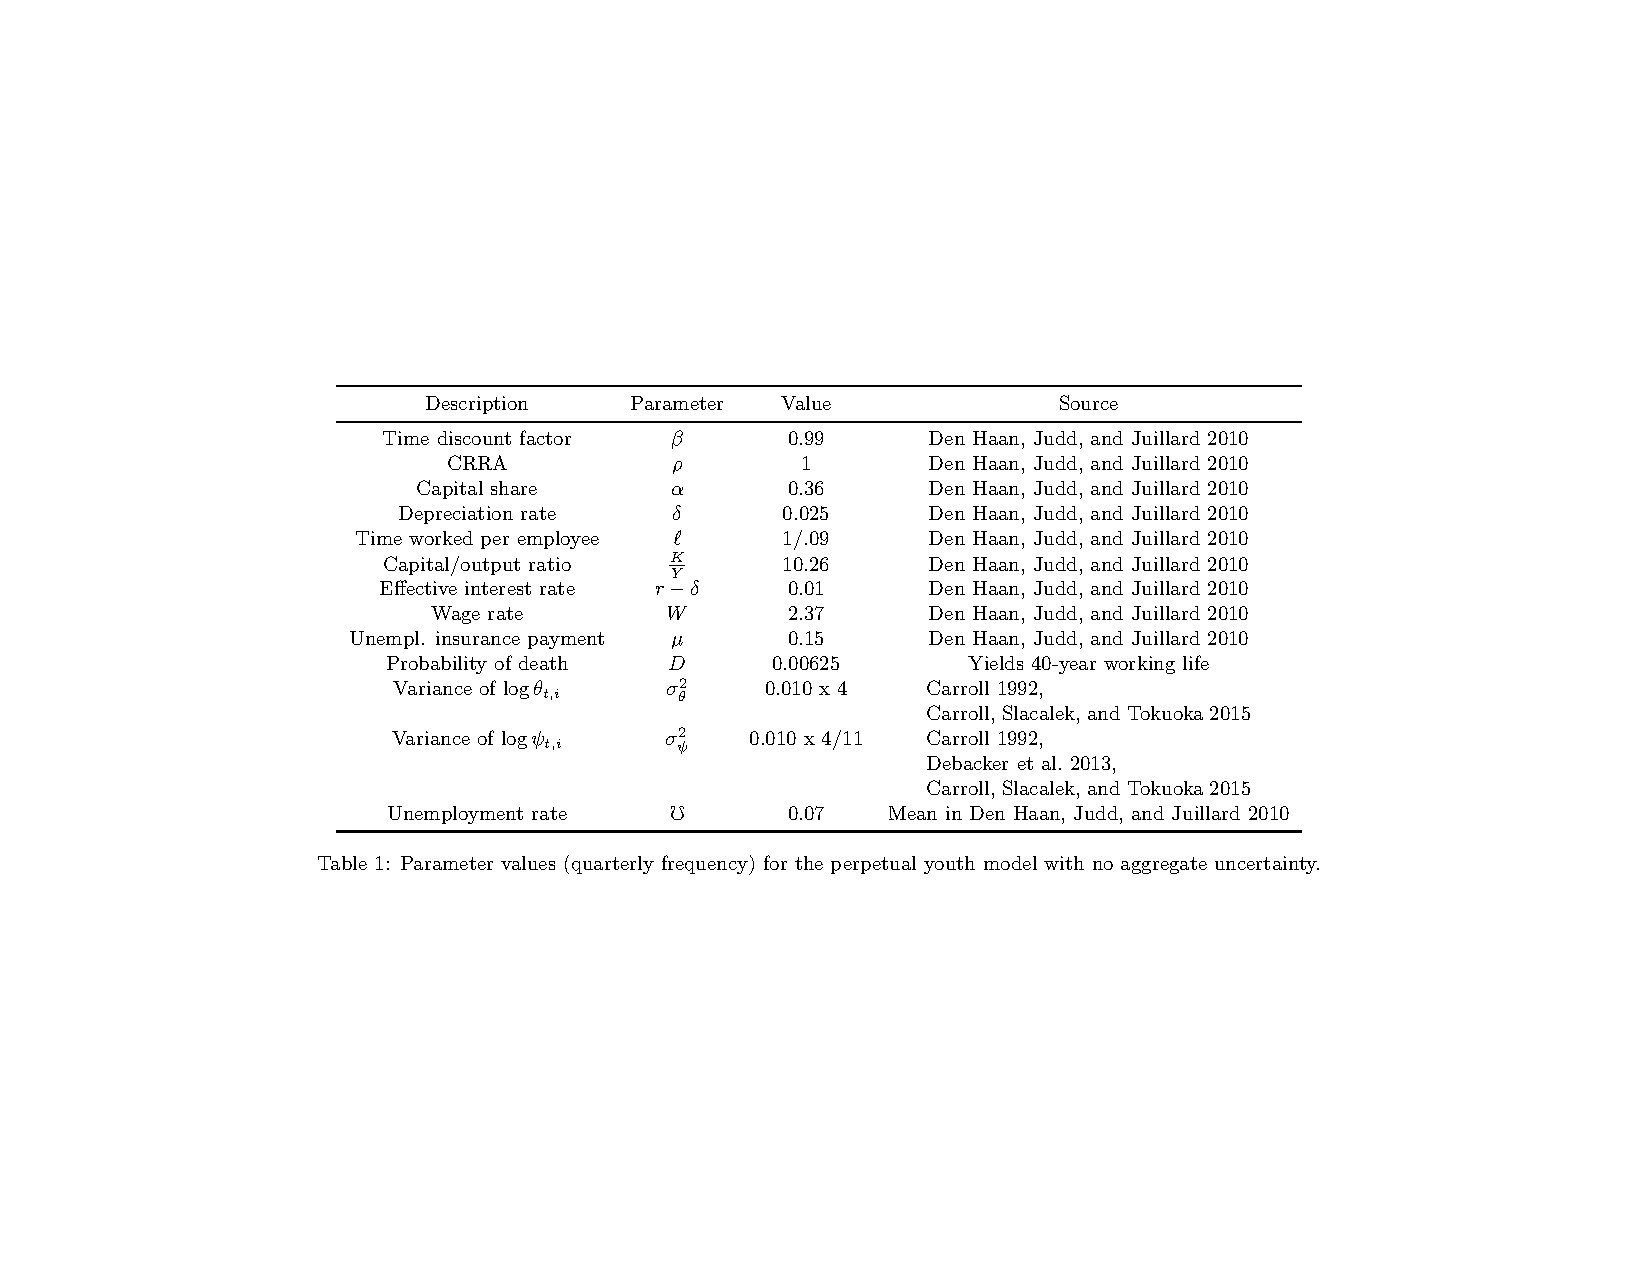
\includegraphics[width=.85\linewidth]{Tables/calibrationPY.pdf}
  \end{figure}
  \vfill

\end{frame}
%%%%%%%%%%%%%%%%%


\begin{frame}{Estimation procedure}

%\vspace{2.5mm}
%Goal: Find $R$ value(s) such that the simulated distribution of wealth best matches \textit{moments} of the household wealth data from the 2004 Survey of Consumer Finances (SCF).

Simulated method of moments (SMM) estimation for $R$.

%\vspace{5mm}
  \begin{enumerate}
  \item No ex-ante heterogeneity: $R$\textit{-point} model
  \par $R$ which matches the capital-to-output ($\frac{K}{Y}$) ratio of $10.26$
  \vspace{2.5mm}
  
  \item Ex-ante heterogeneity: $R$\textit{-dist} model 
  \par \textbf{Uniform distribution} of $R$ matching lorenz targets, given $\frac{K}{Y} = 10.26$ 
  \end{enumerate}
 
  
\end{frame}
%%%%%%%%%%%%%%%%%

\begin{frame}{Estimation procedure with heterogeneity}

\small
\par Empirical lorenz targets using 2004 SCF data \vspace{2mm}

\centering
\begin{tabular}{|c|c|}
\hline
Net worth percentile & Cumulative net worth \\
\hline
20th & -.18\%  \\
40th &  .95\% \\
60th &  5.3\% \\
80th &  17.09\% \\
\hline
\end{tabular}

\begin{flushleft}
\par Optimization problem for the $R$\textit{-dist} model 
\end{flushleft}

\vspace{-7.5mm}
 \begin{eqnarray*}
  \{\grave{R}, \nabla\} = \text{arg}\min_{R, \nabla} \bigg( \sum_{i=20, 40, 60, 80} (w_{i}(R, \nabla)-\omega_i )^{2} \bigg)^{\frac{1}{2}}\\
  &\text{s.t.}& \\
  \frac{K}{Y} = 10.26. %\frac{K_{PF}}{Y_{PF}}. 
\end{eqnarray*}

%try to move "s.t."%

\end{frame}
%%%%%%%%%%%%%%%%%

\section{Results}

\begin{frame}{How good is the match?}
    
    \begin{columns}
    \column{0.5\textwidth}
    \centering
    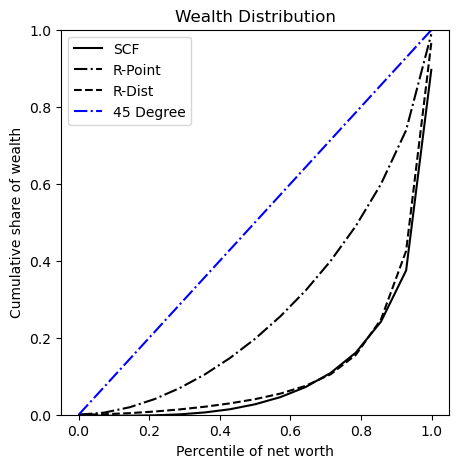
\includegraphics[width=.9\textwidth]{Figures/hetreturns-PYunif.png}
    
    \column{0.5\textwidth}
    \hspace{-5mm}
    \centering
    
    \begin{tabular}{|c|c|c|}

\hline
& $R$-point & $R$-dist \\
\hline
Center & 1.015 & 1.0105  \\
Spread & 0  &  .011  \\
Aggregate MPC & .095 &  .263 \\
\hline
\end{tabular}
    
  \end{columns}
    
\end{frame}
%%%%%%%%%%%%%%%%

\begin{frame}{Revisiting the empirical evidence}

\cite{aflgdmlp20} describe the empirical distribution of returns.



  \vfill
   \begin{figure}
    \centering
    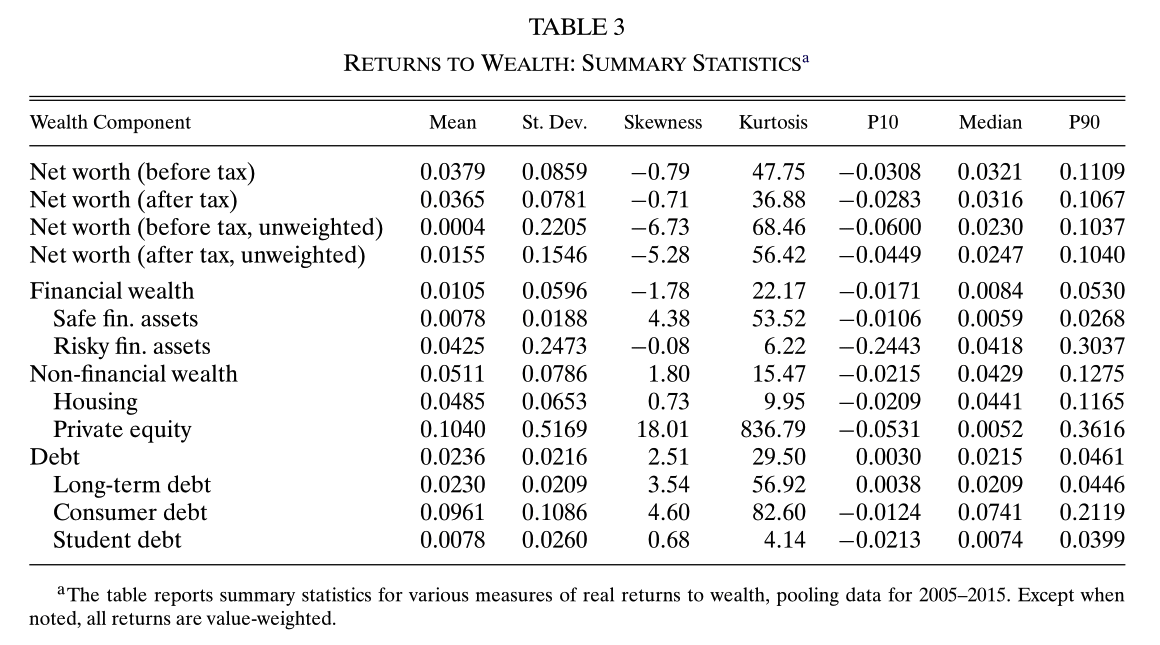
\includegraphics[width=.75\linewidth]{Figures/Fagereng2020Table3.png}
  \end{figure}
  \vfill

\end{frame}
%%%%%%%%%%%%%%%

\begin{frame}{The estimated uniform distribution}
\begin{columns}
    \column{0.5\textwidth}
    \centering
    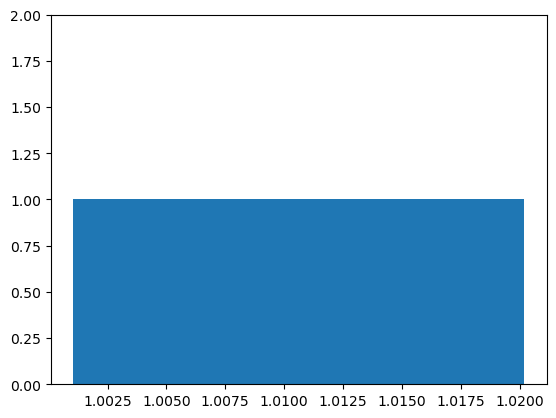
\includegraphics[width=\textwidth]{Figures/estimated-PYunif.png}
    
    \column{0.5\textwidth}
    \centering
    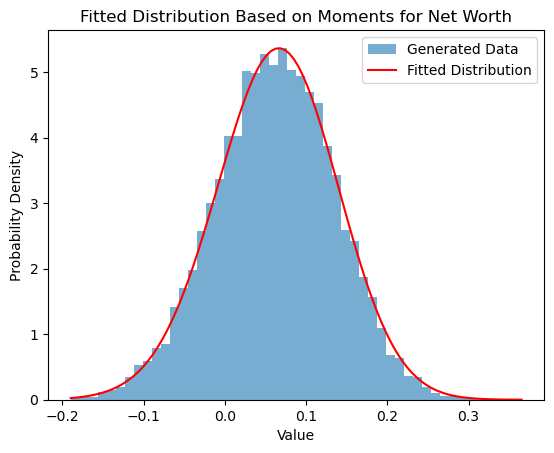
\includegraphics[width=\textwidth]{Figures/Table3QuantileMatchingNetWorth.png}

  \end{columns}
\end{frame}
%%%%%%%%%%%%%%%

\begin{frame}{Matching the data with a lognormal distribution}
  
      \begin{columns}
    \column{0.5\textwidth}
    \centering
    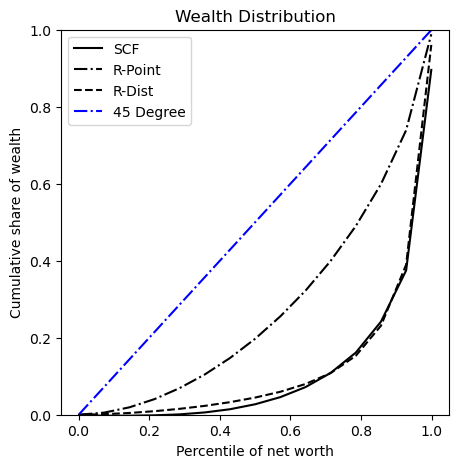
\includegraphics[width=.9\textwidth]{Figures/hetreturns-PYlognrm.png}
    
    \column{0.5\textwidth}
    \hspace{-5mm}
    \centering
    
  \begin{tabular}{|c|c|c|}

\hline
& $R$-point & $R$-dist \\
\hline
Center & 1.015 & 1.0114 \\
Spread & 0  &  .006 \\
Aggregate MPC & .095 &  .241 \\
\hline
\end{tabular}
    
  \end{columns}
  
\end{frame}
%%%%%%%%%%%%%%%%

\begin{frame}{The estimated lognormal distribution}
\begin{columns}
    \column{0.5\textwidth}
    \centering
    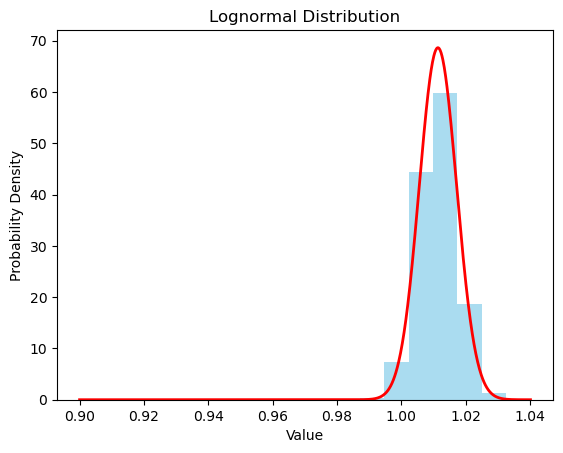
\includegraphics[width=\textwidth]{Figures/estimated-PYlognrm.png}
    
    \column{0.5\textwidth}
    \centering
    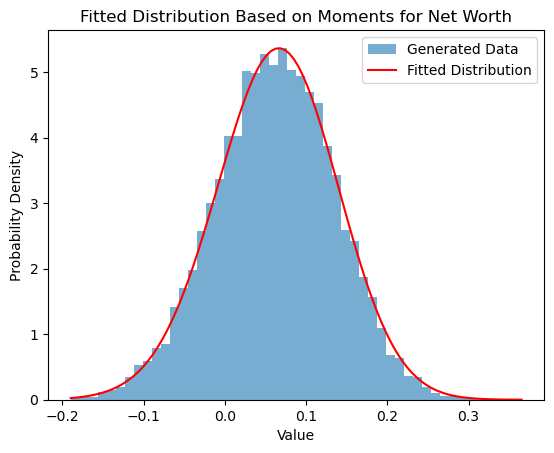
\includegraphics[width=\textwidth]{Figures/Table3QuantileMatchingNetWorth.png}

  \end{columns}
\end{frame}
%%%%%%%%%%%%%%%%%%

%\section{Liquid Asset Holdings}

%\begin{frame}{Matching household data on liquid wealth holdings}

%\par Why liquid wealth?

%\vspace{5mm}
%\par Capital-to-output ratio for liquid wealth to solve the $R$\textit{-point model}: $$\frac{K}{Y}=6.6$$
%\par Lorenz targets for liquid wealth to solve the $R$\textit{-dist model}:

%\centering
%\vspace{2mm}
%\begin{tabular}{|c|c|}
%\hline
%Net worth percentile & Cumulative net worth \\
%\hline
%20th & 0\%  \\
%40th &  .4\% \\
%60th &  2.5\% \\
%80th &  11.7\% \\
%\hline
%\end{tabular}
%\end{frame}
%%%%%%%%%%%%%%%%

%%%%%%%EXCLUDE IQUID WEALTH FOR NOW%%%%%%%%%%%%%%%

%\begin{frame}{How well does the model distribution match the liquid wealth data?}
  
   
    %\begin{columns}
    %\column{0.5\textwidth}
    %\centering
    %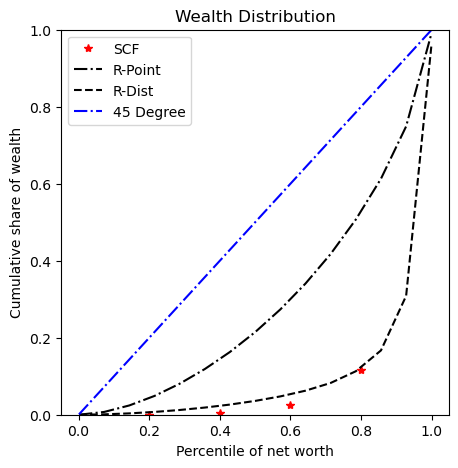
\includegraphics[width=\textwidth]{Figures/hetreturns-PYunif-liqwealth.png}
    
    %\column{0.5\textwidth}
    %\hspace{-5mm}
    %\centering
    
   % \begin{tabular}{|c|c|c|}

%\hline
%& $R$-point & $R$-dist \\
%\hline
%Center & 1.014 & 1.0024  \\
%Spread &0  &  .019 \\
%Aggregate MPC & .108 &  .404 \\
%Lorenz distance & 51.544 & 3.557 \\
%\hline
%\end{tabular}
    
  %\end{columns}
  
%\end{frame}
%%%%%%%%%%%%%%%%

%\begin{frame}{Matching liquid wealth data with an ex-ante lognormal distribution of returns}
    %\begin{columns}
    %\column{0.5\textwidth}
    %\centering
    %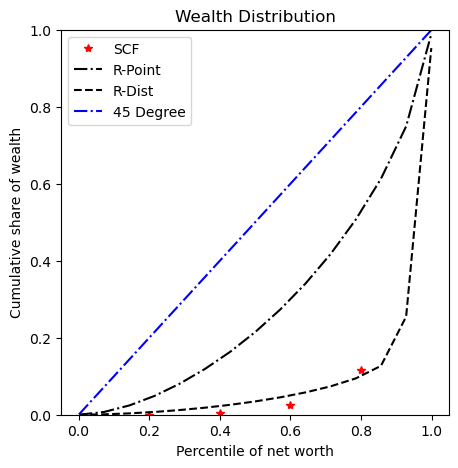
\includegraphics[width=\textwidth]{Figures/hetreturns-PYlognrm-liqwealth.png}
    
    %\column{0.5\textwidth}
    %\hspace{-5mm}
    %\centering
    
   % \begin{tabular}{|c|c|c|}

%\hline
%& $R$-point & $R$-dist \\
%\hline
%Center & 1.014 & 1.0023  \\
%Spread &0  &  .010 \\
%Aggregate MPC & .108 &  .422 \\
%Lorenz distance & 51.542 & 3.629 \\
%\hline
%\end{tabular}
    
  %\end{columns}
%\end{frame}
%%%%%%%%%%%%%%%%

%\begin{frame}{The estimated lognormal distribution of returns for households}
%\begin{columns}
    %\column{0.5\textwidth}
    %\centering
    %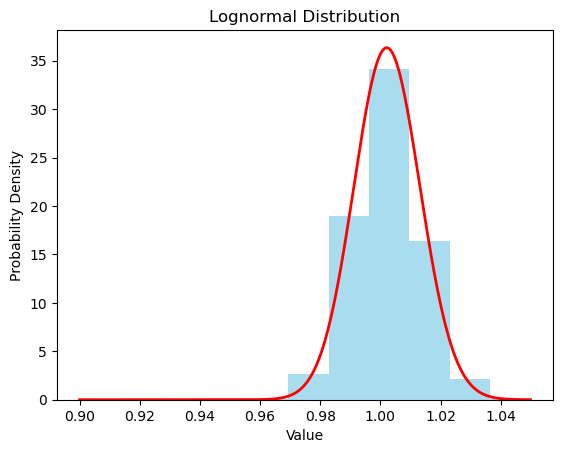
\includegraphics[width=\textwidth]{Figures/estimated-PYlognrm-liqwealth.png}
    
    %\column{0.5\textwidth}
    %\centering
    %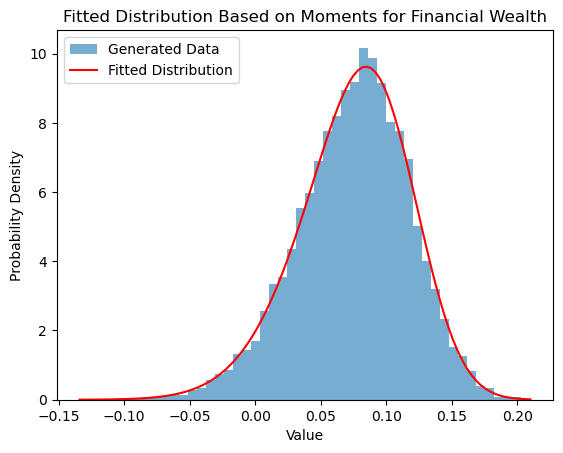
\includegraphics[width=\textwidth]{Figures/Table3QuantileMatchingFinWealth.png}

  %\end{columns}
%\end{frame}
%%%%%%%%%%%%%%%
%%%%%%%EXCLUDE IQUID WEALTH FOR NOW%%%%%%%%%%%%%%%

\subsection{Concluding Remarks}

\begin{frame}{Work to be done}
       
       \begin{enumerate}
       \item Potentially exclude retirement assets in the measure household net worth 
       \begin{itemize}
      \item Private pension wealth is unobservable in the dataset from \cite{aflgdmlp20}
      \item Are there significant differences between retirement asset holdings in the U.S. v.s. Norway?
      \end{itemize}
       \item Run the estimation for liquid wealth
      \begin{itemize}
      \item How close is it to its empirical counterpart (\say{financial wealth})?
      \end{itemize}
      \item Life-cycle version of the model
      \item More recent wealth data from the SCF  
      \end{enumerate}
  
\end{frame}
%%%%%%%%%%%%%%%

\begin{frame}{Future directions for this work}
    \begin{itemize}
    \item Scale dependence of heterogeneous rates of return
    \item Endogenizing differences in the rate of return
    \item Implications of wealth v.s. capital income taxation
      \begin{itemize}
        \item \parencite{Benhabib2008}, \parencite{Benhabib2011}, \parencite{Guvenen2019}
      \end{itemize}
    \end{itemize}
\end{frame}
%%%%%%%%%%%%%%


\begin{frame}[allowframebreaks]{References}
  \printbibliography
\end{frame}

\end{document}




